\chapter{MinION sequencing analysis for viral genomes}\label{ch:concatemers}
\thispagestyle{empty}
\vspace*{\fill}
\epigraph{\emph{A virus can change the fate of the world; power has nothing to do with being tiny or giant!}}
{--Mehmet Murat Ildan}

\clearpage
%%%%%%%%%%%%%%%%%%%%%%%%%%%%%%%%%%%%%%%%%%%%%%%%

This chapter describes another MinION sequencing application for short circular genomes, \EG{} bacterial plasmids or viruses. The text emphasizes the relevant computational methods of the application. 
This study exploits the excessive length of nanopore reads and their potential to harbor multiple copies of small-sized viral DNA sequences. These genomes, given sufficient coverage depth, can be reconstructed by a high-resolution consensus calling of the single molecule 
Even though this study does not present real-time results from the device, it is straight-forward to adapt such pipeline using the developed modules since they operate rapidly in a read-by-read manner.

The analyses reported in this chapter come solely from my contribution to a joint project studying plant viral genomics. 
The lab works, including but not limited to DNA extraction, amplification as well as library preparation and sequencing steps were established independently thus will not be described in details.
The data has not yet been published but permission to document part of the preliminary research findings for this thesis has been granted by all collaborators.
\section{Introduction}
There have been attempts to sequence bacterial plasmids using MinION device as part of a whole genome assembly~\cite{Lemon2017M15,Wick2017M12} or in exclusively studies~\cite{Li2018M13,Lu2018plamids}. As mentioned earlier, studying the whole structure of \emph{replicons} is important as they are responsible for the horizontal gene transfer between strains, \EG{} the dissemination of AMR factors in \emph{superbugs}.
At the same time, it is critical to understand the mechanism of viral transmission and evolution in real-time to monitor and control  epidemics~\cite{GardyLR2015,AndersenSM2015,HolmesDR2016,DudasCB2017}.
As a result, nanopore sequencing for viral samples has already been employed in clinics or even in the field during outbreaks, \EG{} influenza~\cite{Wang2015minion}, Ebola~\cite{QuickLD2016} or Zika~\cite{Quick2017GP} viruses.

The ONT MinION benefits sequencing short genomes, such as viruses, in many ways especially in terms of genome assembly. 
In fact, we regularly obtain nanopore reads that cover the whole length of the circular IncP-$\alpha$ plasmid RP4 (around $60$kpb long) genomes~\cite{Lu2018plamids}, which significantly assist in the assembly phase.   
Even without associated Illumina data, nanopore data can generate results with decent quality after consensus calling thanks to sufficient high coverage~\cite{Vaser2017racon}.
The multiplexing method is usually applied to reduce the costs and increase the scale of microorganisms study of interests~\cite{Quick2017GP}.

Here another approach is presented for viral sequencing using ONT platform. A special amplification technique is employed to increase the copy numbers of the whole circular DNA molecules before being subjected to the sequencing step by MinION and relevant computational task for subsequent assembly.

\paragraph{Rolling-circle DNA amplification}
PCR is the most widely used amplification method for many organisms in general but for this study, we employed different whole genome amplification technique in order to obtain longest sequences possible for MinION sequencing.
The cloning method is known as rolling-circle amplification (RCA), a one-step whole-genome multiplication that has been applied for small circular DNA molecules, especially virus families~\cite{Rector2004rca14,Inoue2004rca28,Schubert2007rca30,Knierim200rca31,Shepherd2008rca32,Haible2006rca33,Homs2008rca34}.

\begin{figure}[!hpt]
\centerline{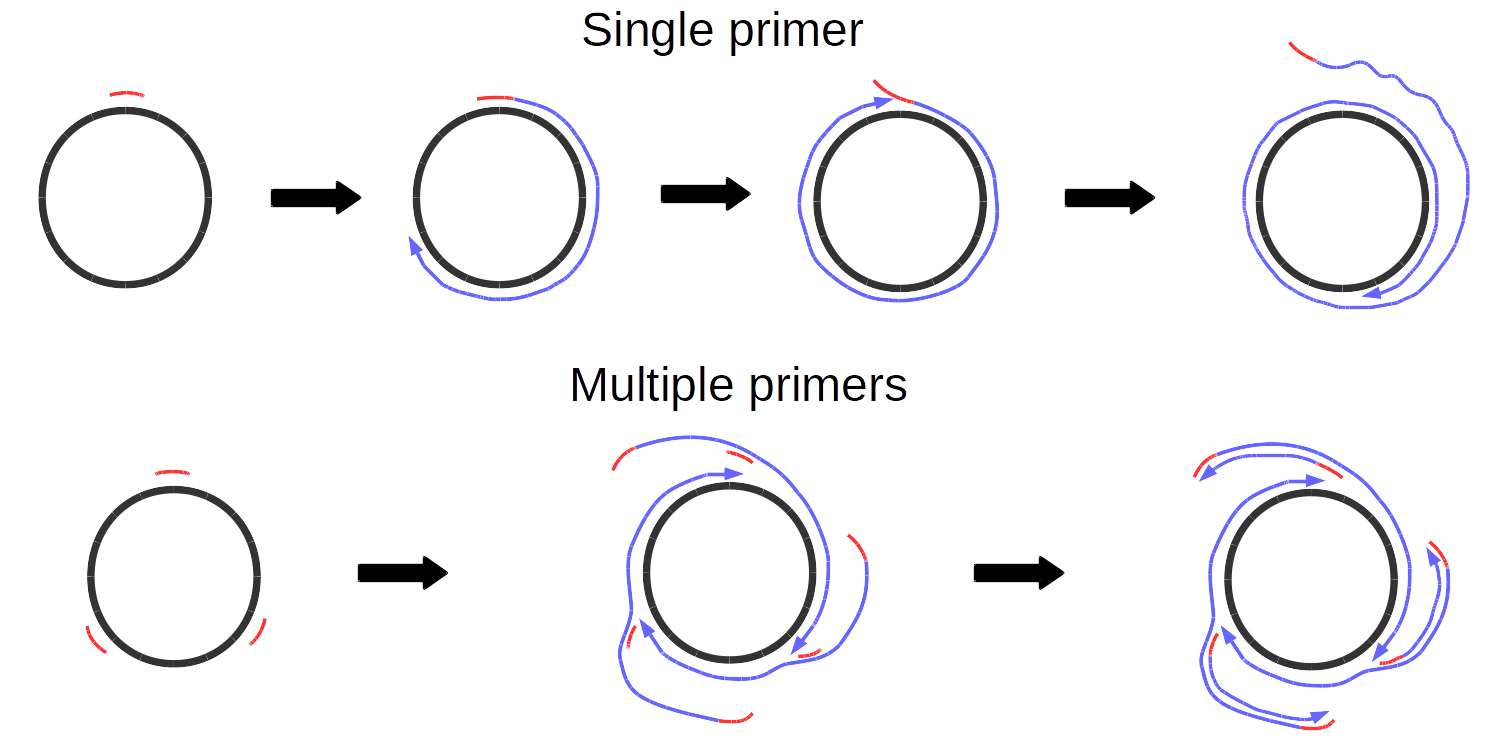
\includegraphics[width=0.9\textwidth]{images/rca.png}}
\caption[Rolling Circle Amplification]{General mechanism of Rolling-Circle Amplification. Figure is adapted from~\cite{Johne2009rca} under Elsevier license (attached at the end of this thesis). Primer sequences are highlighted in red, the circular genome subjected for amplification is in black and the synthesized clones are in blue.}
\label{fig:concat_rca}
\end{figure}

The basic principle for RCA is shown in Figure~\ref{fig:concat_rca}~\cite{Johne2009rca}.
On top is an example of the process with only one imaginary primer binding to a template circular. The synthesis starts from this point and move across the whole length of the molecule in the complementary direction as being guided by the DNA polymerase  \emph{phi29} of bacteriophage \emph{Baccilus~subtilis}.
Due to this particular enzyme's features, the incorporation can continue passing the binding site whilst the newly synthesized strand being displaced from the track.
Depending on the size of the template circle, the copying process can go several rounds, resulting in elongated molecules consisting of multiple copies of the original.
From the diagram in the bottom of Figure~\ref{fig:concat_rca}, multiple random primers are used for the amplification as it should usually be in practice. In this case, the abundance of primers from the reaction mixture can bind to the displaced strand and trigger additional syntheses, creating the branching patterns of the cloning process.

The RCA products are called concatemers as they are long concatemeric molecules consisting of consecutive copies of the target DNA sequence. Normally, restriction enzymes are used to chop them into separated monomers before taking further steps. For our method, concatemers are directly sequenced by MinION and computational methods are used afterward to detect such patterns.
\paragraph{Viral samples}
The viral genomes used in this study belonged to the plant infectious family \emph{Caulimoviridae}, or \emph{caulimovirids} with size varied around $7$-$9$Kbp.
Amongst nine genera detected~\cite{Geering2010ST,Mollov2013LZ}, two of them were investigated, namely \emph{Badnavirus} and \emph{Caulimovirus}, represented by \emph{Banana streak MY virus} (BSMYV) and \emph{Cauliflower mosaic virus} (CaMV) respectively.

\section{Bioinformatics analyses}
\subsection{Data description}
A multiplex sequencing has been conducted for 4 samples with the Rapid Barcode Sequencing kit. The barcode assignment is given in Table~\ref{tab:viral_samples}.
\begin{table}[!ht]
\centering
\caption{Viral samples subjected to MinION barcoding sequencing}
\label{tab:viral_samples}
\begin{tabular}{lllrr}
\hline
\toprule
\textbf{Barcode} & \textbf{Sample} & \textbf{Description} & \textbf{Pass reads}  & \textbf{N50}    \\
\hline
\rowcolor{Gray}
08                  & CaMV+              & \emph{Cauliflower mosaic} virus  &   14,385   &      6,707 \\
09                  & BSMYV+             & \emph{Banana streak MY} virus    &   3,389   &   8,178   \\       
\rowcolor{Gray}
10                  & BSMYV-             & \emph{Banana streak MY} virus, negative control     &   4,653   &  6,023   \\
12                  & CaMV-              & \emph{Cauliflower mosaic} virus, negative control     &   9,942   &  4,919   \\\hline
\end{tabular}
\end{table}

\subsection{Reference-based detection of concatemers}
Raw signal data from MinION were base-called and demultiplexed by \albacore{} version 2.1.0. This resulted in 4 DNA sequence files corresponding to 4 barcoded samples, only pass reads from those sequences were used for further analyses.

\paragraph{Work flow} Due to the application of rolling circle amplification, each long read is expected to contain more than one copy of the virus DNA, potentially sitting next to each other in a \emph{concatemer}. We create an in-house pipeline to detect and extract the \emph{monomer} sequences out of the reads to build their consensus as shown in Figure \ref{fig:concat_ref_workflow}.

\begin{figure}[ht]
\centerline{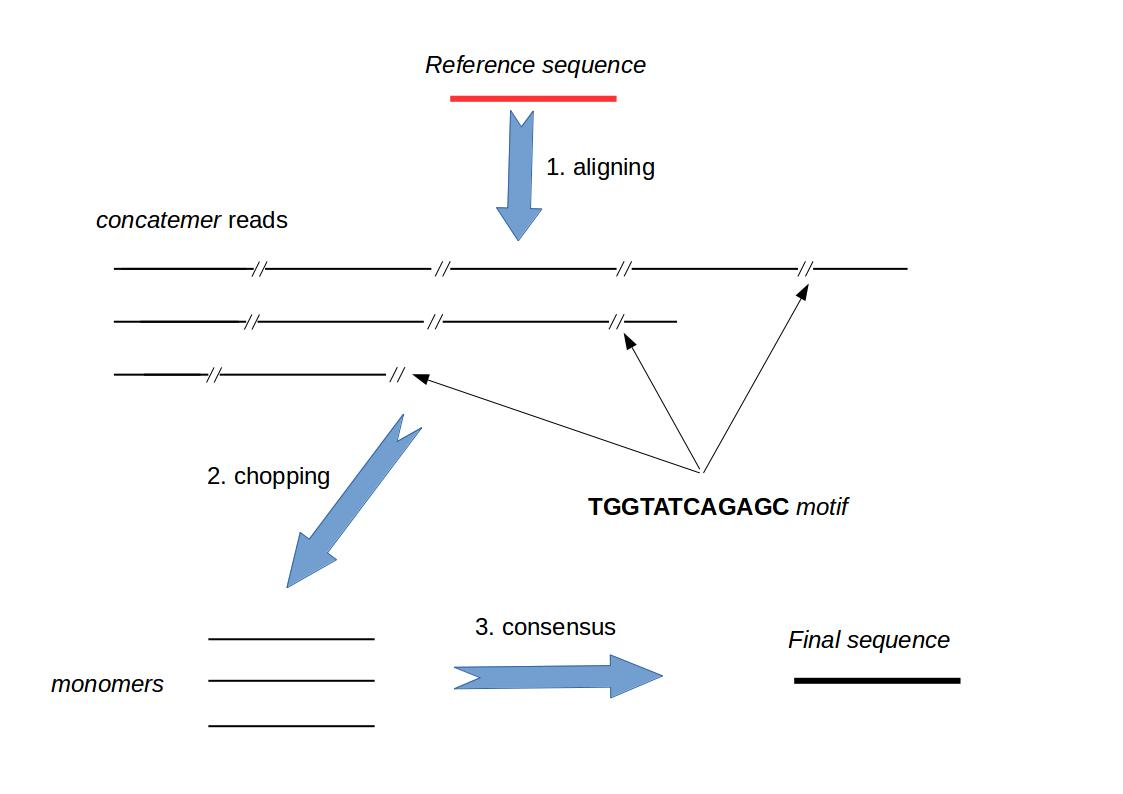
\includegraphics[width=0.9\textwidth]{images/concatemer.jpg}}
\caption{Pipeline to reconstruct viral genome sequences from MinION long reads.}
\label{fig:concat_ref_workflow}
\end{figure}

In more details, the pipeline is implemented in the following steps: 
\begin{itemize}
\item[1.] align nanopore reads to the corresponding reference by \minimap{}~\cite{Li2016} version 2.11-r797 and keep only the ones covering $>80\%$ of the target; then induce locations of monomer on each reads based on the alignments.
\item[2.] for each monomer inferred, scanning for the nearest hit to the tRNA$^{Met}$ 12 nucleotides motif \textbf{TGGTATCAGAGC} where the DNA synthesis is primed in \emph{Caulimovirids} replication cycle~\cite{Bhat2016badnaviruses,Sukal2018characterization}. Those loci are then used as final breakpoints for a later chopping step to extract monomers.
\item[3.] build consensus sequence on those extracted monomers by \racon{}~\cite{Vaser2017racon} version 1.2.1.
\end{itemize}

\paragraph{Align to the reference}
Figures \ref{fig:bc08} and \ref{fig:bc09} show the read length histogram of only mapped reads from nanopore data of barcode 08 and 09 respectively. Two negative control samples (barcode 10 and 12) returned no hits when aligned to their corresponding reference thus not shown. As can be observed, CaMV virus (barcode 08) has richer sequencing data compared to BSMYV sample (barcode 09).
\begin{figure}[!ht]
\centering
\subfloat[Mapped reads from barcode 08\label{fig:bc08}]{
	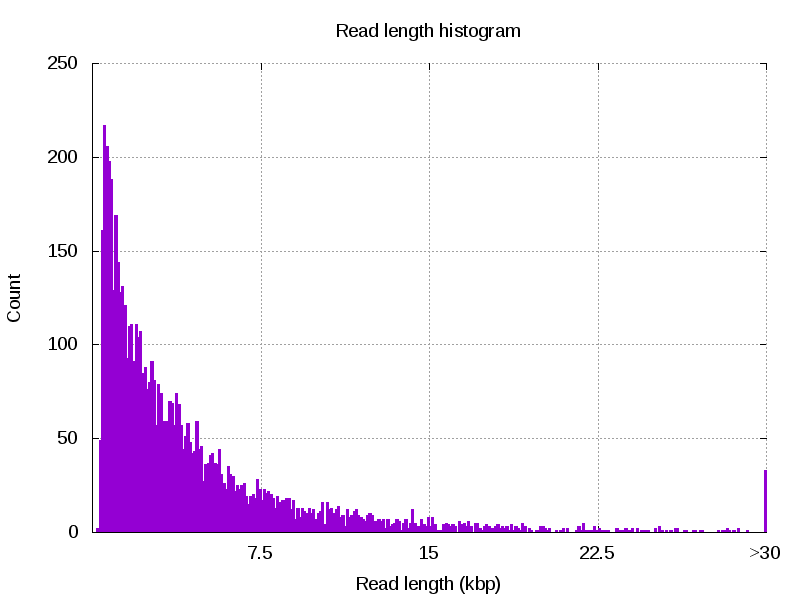
\includegraphics[width=.5\textwidth]{images/barcode08.png}
}
~
\subfloat[Mapped reads from barcode 09\label{fig:bc09}]{
	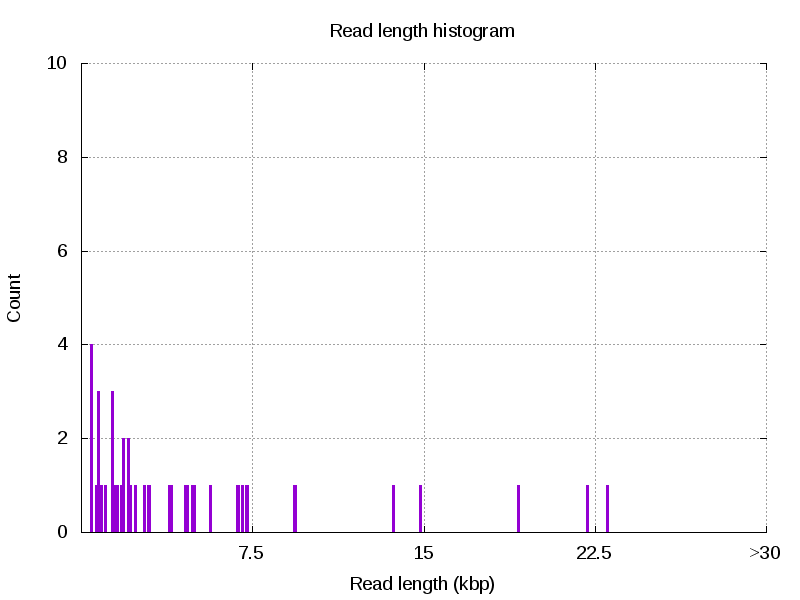
\includegraphics[width=.5\textwidth]{images/barcode09.png}
}
\caption{Mapped read length histogram of barcode 08 and 09.}
\label{fig:concat_map}
\end{figure}

\paragraph{Concatemer extraction}
Chart \ref{supp_fig:concat_count} presents the number of $k$-concatemers (concatemers with exact $k$ monomers extracted) for each positive sample (barcode 08 and 09). 
The longest concatemer detected was a 7-concatemer of CaMV DNA sequence. 
There was also one 6-concatemer and one 4-concatemer from this sample. 
In addition, the numbers of detected $k$-concatemers for \emph{Cauliflower mosaic} virus were more than 1 for $k=3$ (2 reads) or $k=2$ (6 reads).
Monomer reads made up the most abundance group with 33 CaMV sequences and 5 BSMYV sequences.
There were no other concatemers detected for the latter sample.

The extraction step generated in total $68$ and $5$-folds coverage of monomers respectively for barcode 08 and 09. By using these monomer sequences, we can pile them up and call the consensus sequence out of the nanopore data. The obtained sequence coverage played a critical role for the accuracy of the result: for barcode 08, the consensus was $99.5\%$ identical to its reference while it was only $93.72\%$ in case of barcode 09. 

\subsection{Reference-free method}
Assuming no references are given, the duplication of a DNA sequence in a nanopore read can still be detectable by using self-alignment to study the repeat pattern.
A proposed approach to investigate periodic repeat patterns is to use auto-correlation function (ACF) in digital signal processing (DSP) technique.
Similar DSP-based methods have been developed for fast biological sequence alignment and repeat detection \cite{Rockwood2005crosscorrelation,Ravi2007tandem}.
Here I present another application of signal processing techniques to detect the concatemers of the aforementioned viral sample using nanopore data. 
Tools are developed to work on both base-called and raw signal sequences.
For better demonstrating purpose, analysis result from the longest 7-concatemer read (from barcode 08 sample) is described without loss of generalization.

\subsubsection{Auto-correlation function}
Given an infinite sequence of discrete signals $S=\ldots s_1 s_2 \ldots s_k \ldots$ where $S(i)=s_i$ , its ACF $f(n)$ is defined as the cross correlation to itself
\begin{equation}
 f(n)=\sum_{k}{s_k\ast s_{k-n}}   
 \label{eq:acf}
\end{equation}
where $\ast$ operator returns a similarity score when compare two operands, \EG{} complex conjugate for $s(i) \in \mathbb{C}$~\cite{Rockwood2005crosscorrelation}, and $n$ stands for the lag value. By increasing this value, we have a sliding dot product between the signal vector with itself which in expect give peaks when repeat parts of the sequence are overlapped as demonstrated in Figure~\ref{fig:concat_acf}. Note that for every signal sequence $S$, there is always a peak at $n=0$ as a result from self-overlapping. In addition, the ACF values are symmetric with regard to this center value.
\begin{figure}[ht]
\centerline{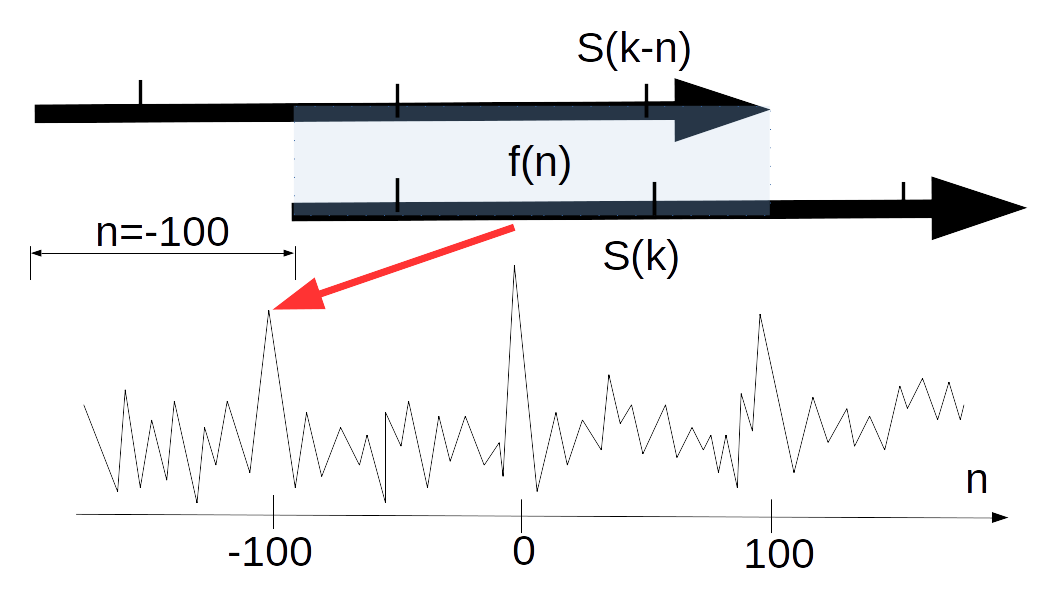
\includegraphics[width=0.7\textwidth]{images/acf.png}}
\caption[Example of ACF sliding dot product for a sequence with two repeats]{Example of ACF sliding dot product for a sequence with two repeats. The plots shows 3 dominating peaks corresponding to $n=-100, n=0, n=100$.}
\label{fig:concat_acf}
\end{figure}

In fact, the signal sequence to process is definite: $S=\{s_i\}, i=1 \ldots L$ for sequence with length $L$. Out of range values are normally zero padded $s_j \equiv 0 \: \forall j \leq 0,j > L$ or duplicated so that $s_i \equiv s_{i+n \times L} \: \forall n \in \mathbb{Z}$. In this study, the former filling method is used.

The following content will focus on ACF-based attempts in determining the concatemeric pattern of nanopore long reads.
Firstly, in the next section, a straightforward strategy will be employed  directly on the base-called sequence of nucleotides. The sliding dot product algorithm for the time-domain signal, together with a simple filter will be implemented initially. 
This simple but applicable method would serve as a proof-of-concept for the idea of using DSP technique to the problem.
After that, we introduce a more robust method that allows fast calculations not only on the DNA sequences, but also on the raw squiggle signals from the underlying ONT sequencing process. 
The ability to operate quickly per read would enable the concatemers detection to work in a streaming fashion so that it can be integrated in a real-time pipeline as aforementioned.

\subsubsection{Concatemers detection protocol using DSP}
To apply DSP algorithm, the first step is to convert the nucleotides sequence into appropriate digital signal.
Given a DNA sequence, we have $S(i)=s_i \in \{A,C,G,T\} \: \forall i \in \mathbb{N}$. A straightforward conversion is to map letters to their corresponding numerical values, \EG{} $\{1,2,3,4\}$ respectively.
Consequently, the $\ast$ operator from Equation~\ref{eq:acf} can be simply adapted to the Kronecker delta function
\[
s_i \ast s_j \equiv \delta_{s_i,s_j} = \left\{
\begin{array}{ll}
0     &  if \: s_i = s_j\\
1     &  if \: s_i \neq s_j
\end{array}
\right.
\]
As shown in Equation~\ref{eq:nkdf}, the ACF values are normalized by the overlap length to alleviate the position-dependant behaviour of the function that is important to locate peaks that represent monomer overlaps in next step. 
Due to the errors (indels/mismatches) of MinION sequence data, these overlaps are not aligned perfectly as of one-to-one mapping of base pairs but rather scattered hits along the overlapped region.
This results in a `group of nearby spikes' rather than a single prominent peak, making it more difficult to locate exact coordinates of monomers in the read. 
For that reason, a low-pass filter (LPF) is needed to help reduce the noises, or \emph{smooth} the signal before further analysis. 
Primarily, we use \emph{running average} with a fixed window size ($ws$) of nearby values for such task. 
We set the window size equal to 10 for this scenario. 

Overall, for this case, we investigate the signal of the normalized Kronecker delta function (NKDF) as shown in Equation~\ref{eq:nkdf}
\begin{equation}
\label{eq:nkdf}
f(n) = \frac{\displaystyle \sum_{i=1}^{L}{\delta_{s_i,s_{i-n}}}}
            {\displaystyle L-|n|}
            , n \in (-L;L)
\end{equation}
then apply the running average filter on it
\[
\overline{f(n)} = \frac{\displaystyle \sum_{i=-ws/2}^{ws/2}{f(n+i)}}
            {\displaystyle ws}
\]

\begin{figure}[!ht]
\centering
\subfloat[ACF for a random DNA sequence\label{fig:acf_random}]{
	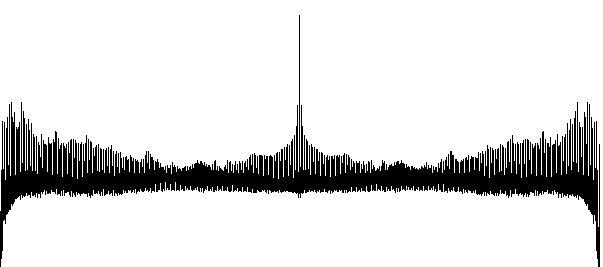
\includegraphics[width=.49\textwidth]{images/concatemer-random.png}
}
~
\subfloat[ACF for the 7-concatemer read\label{fig:acf_7cm}]{
	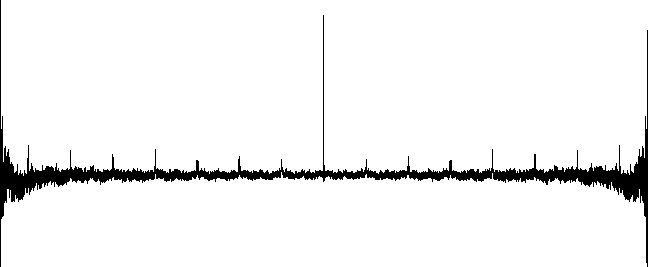
\includegraphics[width=.49\textwidth]{images/concatemer-7cm.png}
}
\caption[ACF values for a random read versus the 7-concatemer detected]{ACF values for a random read (\ref{fig:acf_random}) versus the 7-concatemer detected (\ref{fig:acf_7cm}).}
\label{fig:concat_acf_dna}
\end{figure}

Figure~\ref{fig:concat_acf_dna} presents the result signal for the detected 7-concatemer versus a random synthetic read with similar length.
According to the plots, there is only one distinct peak from the ACF signal of the random read which reflects the trivial case of self-alignment. On the other hand, from the longest concatemer read available, we can observe 7 clear peaks on each side of the symmetric squiggle representing the same copy number of the viral monomer.
These peaks are possibly identified by a peak picking algorithm which can determine the significant local maxima located across the range with similar distances. 

On the other hand, the formula \ref{eq:nkdf} implies greater variance of the signal values toward the ends of the range $(-L;L)$ due to fewer overlap data points involved. This tailing issue would hinders the algorithm to locate the monomers at two ends of a read. This effect can be observed from Figure~\ref{fig:acf_7cm} where the squiggles become more diverse leaving further the center lag ($n=0$).
For that reason, the peak picker will start the scan from $n=0$ to either side for distinct spikes of higher confident and determine the period before reaching the noisy peaks toward the ends.
Figure~\ref{supp_fig:concat_acf_dna} from the Appendix gives more examples of ACF-induced signals for several other $k$-concatemers using this calculation method. Similarly,  in all cases the fluctuations at the ends of ACF graphs are plotted beside the `genuine' maxima. This introduces difficulties to detect `real' hits close to the ends especially when $k=1$ as we have no other peak for comparison.

In general, via above experiment, the DSP approach utilizing ACF-based estimation has been proved to be feasible to detect the concatemeric pattern of nanopore RCA reads.
However, there are several points needed to be further developed and improved from this protocol to be able to work in an applicable pipeline.
The most important task is to optimize the algorithm to reduce the running time. The current sliding method takes $\mathcal{O}(L^2)$ time for a read of length $L$.
Even though it is relatively reasonable for viral concatemers of medium length ($\simeq 50$Kbp), it would become time-consuming to process reads with high copy numbers which are favoured and aimed for in this study.
Also, the turn-around speed per read is critical in real-time analysis, not to mention the desired application at the level of sequencing raw signal from the very pre-basecalling stage.
Another essential operation is a robust LPF mechanism since the simple moving average method is unable to comprehensively remove the high-frequency noises from the target signal. Lastly, a peak picking algorithm is needed to spot the periodical maxima and chop the repeat sequence at those breakpoints into monomers of interest.
All of those steps will be addressed in the following section.

\subsubsection{Rapid method to detect concatemeric signal}
\paragraph{Generalized problem for real signal data.}
While Kronecker delta function is fast to calculate, it is only suitable for sequences of discrete, categorical values \EG{} DNA letters. 
Nanopore raw signal for a read is given as a series of real values of electrical current sampled thousands times per second when the biological molecular transiting through the pore. 
Processing concatemers at raw signal level before base-calling would accelerate the whole pipeline to a new level, as well as improving the quality of signal for the next stage. 

From this context, the sequence $S,\: S(i)=s_i \in \mathbb{R} \: \forall i$ would have ACF written as
\[
 f(n)=\sum_{k}{s_{k}s_{k-n}}   
\]
where the $\star$ operator in Equation~\ref{eq:acf} is replaced by the multiplicity in $\mathbb{R}$ instead of the previous Kronecker delta function for discrete values of $\mathbb{Z}$.
Due to the symmetric property of ACF, only the right half of the range will be considered instead of the whole plot as demonstrated in Figure~\ref{fig:concat_acf_dna}, corresponding with lag from $0$ to $L-1$. The trivial peak of self-alignment thus locates in the very first element of the array.
\paragraph{Rapid estimation method for normalized ACF signal}
Calculation of ACF function given above is straight-forward and efficient using Fast Fourier Transform (FFT)~\cite{Gentleman1966FFT,Van1992FFT,Heideman1984FFT} with complexity $\mathcal{O}(L\log{L})$.
However, to additionally normalize the signal while maintaining the speed aspect of the algorithm is not a trivial task.
To achieve such goal, the Normalized Square Difference Function (NSDF)~\cite{Mcleod2005tartini} is implemented. This function can be calculated as shown in Equations~\ref{eq:nsdf}.
\begin{equation}
\label{eq:nsdf}   
\begin{array}{rr}
h(n)=& 1-\frac  {\displaystyle \sum_k{(s_k-s_{k-n})^2}}
                {\displaystyle \sum_k{(s_k^2+s_{k-n}^2})} \\
    =& \frac{\displaystyle \sum_{k}{2s_{k}s_{k-n}}}
            {\displaystyle \sum_k{(s_k^2+s_{k-n}^2})}\\
    =& \frac{\displaystyle 2f(n)}{\displaystyle g(n)}\\
\end{array}
\end{equation}
The values of $h(n)$ would fall in $(0,1]$ with $\forall n$, representing a normalized measure of proximity between $S$ and its $n$-delay signal. 

\begin{algorithm}[H]
\DontPrintSemicolon
\KwIn{Time-domain sequence signal $S$ of lenth $L$}
\KwOut{NSDF signal $H$}
\SetKwFunction{ACF}{ACF} 
\SetKwProg{Fn}{Function}{:}{}
\Fn{\ACF{$S$, $R$}}{ 
    $R:=\mathtt{fftForward}(S)$ \tcp*{Convert signal to frequency domain by FFT}
    $R[i]:=R[i] \star R[i]$, $\forall i=0 \ldots (L-1)$  \tcp*{complex conjugate element-by-element}
    $R:=\mathtt{fftReverse}(R)$ \tcp*{Convert back to time domain by reverse FFT}
    \KwRet\;
}
\SetKwFunction{SS}{SS} 
\SetKwProg{Pn}{Function}{:}{}
\Pn{\SS{$S$, $M$}}{ 
    $SS[i]=S^2[i]$, $\forall i=0 \ldots (L-1)$ \;
    $M[0]=2*\mathtt{sum}(SS)$ \tcp*{get sum of all elements in $\mathtt{SS}$}
    $M[i]=M[i-1]-SS[i-1]-SS[L-i]$, $\forall i=1 \ldots (L-1)$ \tcp*{update incrementally}
    \KwRet\;
}
\Begin{
\ACF{S,R} \tcp*{calculate ACF and assign to R}
\SS{S,M} \tcp*{calculate lag sum square and assign to M}
$H[n]=\frac{\displaystyle 2R[n]}{\displaystyle M[n]}$, $\forall n=1 \ldots (L-1)$ \tcp*{calculate NSDF as in Equation~\ref{eq:nsdf}}
\Return{$H$}
}
\caption{Algorithm to calculate the NSDF by using FFT.}
\label{algo:nsdf}
\end{algorithm}
More than that, this function is determined by $f(n)$ and $g(n)$ which can be both measured rapidly by using FFT (using $\mathtt{JTransform}$~\cite{Eichelberger2002jtransform}, a Java library for DSP) and incremental calculation as shown in Algorithm~\ref{algo:nsdf}.

\paragraph{LPF with Blackman windowing function.}
%http://www.labbookpages.co.uk/audio/firWindowing.html#windows
The plain moving average method is helpful to show the trend of the overall signal but not sensitive enough to completely remove the noises encountered.
Figure~\ref{supp_fig:concat_acf_raw} in the Appendix plots the NSDF of the 7-concatemer read with large smooth window sizes of $10,000$ and $20,000$. 
As a peak scanning method is sensitive to abundant of local optima, a `smoother' transition is expected via a signal filtering step. 
For that reason, a finite impulse response (FIR) filter by windowing is implemented.
\begin{figure}[!hpt]
\centering
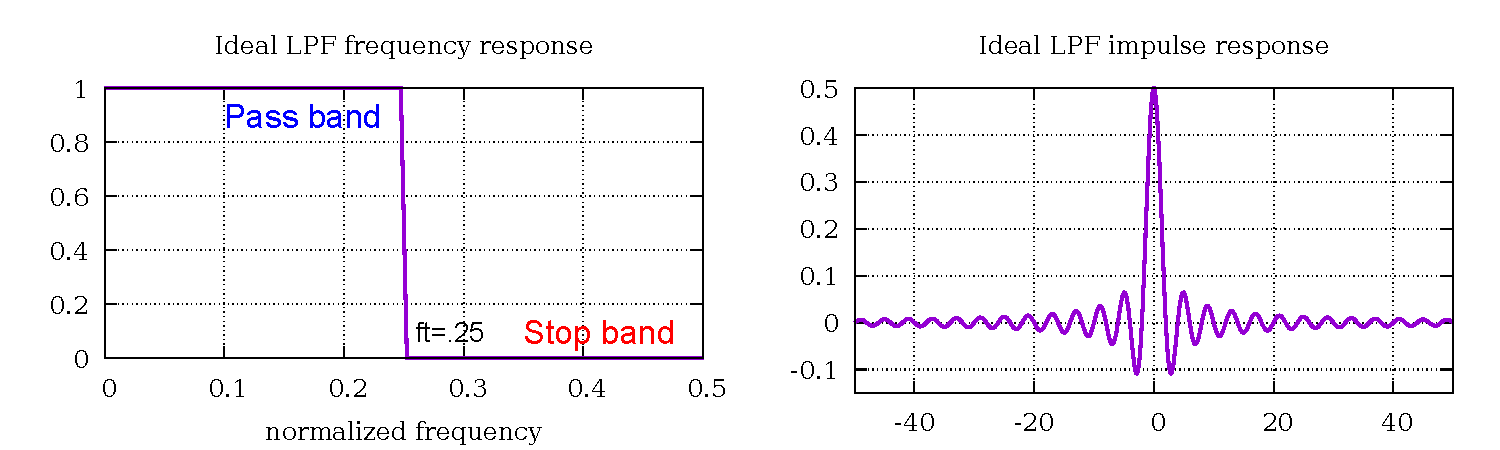
\includegraphics[width=\textwidth]{images/fir.pdf}
\caption{Example of ideal LPF at $f_t=0.25Hz$ and its corresponding impulse response.}
\label{fig:fir}
\end{figure}

Figure~\ref{fig:fir} gives example for an ideal LPS with transition (cutoff) frequency $f_t=0.25$. The left plot presents the frequency response of the filter in frequency domain (normalized with respect to the sampling frequency). In this perfect scenario, a brick-wall filtering is expected when any frequency values below $0.25Hz$ would pass and all higher components are stop.
This system would have an equivalent impulse response as shown on the right plot, given by function $\mathtt{IRF}$:
\[
\mathtt{IRF}(x) = 2f_{t}\ sinc(2\pi f_t x)
\]
where $sinc(x)$ is the \emph{sine cardinal} function
\[
sinc(x) = \left\{
\begin{array}{ll}
\frac{\displaystyle \sin{x}}{\displaystyle x}     &  if \: x \neq 0\\
1     &  if \: x=0
\end{array}
\right.
\]
In practice, to implement a finite impulse response LPF, only a window of the shifted sinc function is sampled for a finite number of filter weights. 
We set this window's length, or filter length, as the length of signal $L$. 
\begin{equation}
\label{eq:sinc}
\mathtt{IRF}(n) = \left\{
\begin{array}{ll}
\frac{\displaystyle \sin{[2\pi f_t (n-\frac{M}{2})}]}{\displaystyle \pi (n-\frac{M}{2})}     &  if \: n \neq \frac{M}{2}\\
2f_t     &  if \: n=\frac{M}{2}
\end{array}
\right.
\end{equation}
where $M$ is the filter order, defined as $M=L-1$.

Furthermore, to reduce the ripple from the ringing artifact due to crude approach of truncating the infinite ideal impulse response~\cite{Smith1997DSP,Bankman2008image}, we apply Blackman windowing~\cite{Harris1978use,Blackman1958measurement} instead of a rectangle window ($w(n)=1$) on the IRF values.
\begin{equation}
\label{eq:windowing}
w(n)=0.42-0.5\cos{\frac{\displaystyle 2\pi n}{\displaystyle M}}+0.8\cos{\frac{\displaystyle 4\pi n}{\displaystyle M}}
\end{equation}
Overall, to apply the LPS with Blackman windowing on the NSDF signal, we follow the steps below.
\begin{itemize}
    \item[(1)] Calculate the weights of the LPF as a function of cutoff frequency $f_t$ as in Equation~\ref{eq:sinc}
    \item[(2)] Multiply the result with the windowing calculated in Equation~\ref{eq:windowing}
    \item[(3)] Apply FFT for the result filter values.
    \item[(4)] Calculate FFT of the NSDF and multiply its values element-by-element to the filter values in the frequency domain.
    \item[(5)] Calculate the reverse FFT to get the result in the time domain.
\end{itemize}


The cutoff frequency (before being normalized) is empirically set as $100Hz$ assuming that a $100$-times RCA duplication is virtually impossible or due to process's artifacts.
This threshold can be set more stringent with knowledge about specific reference genome size and obtained sequencing read length. 
Figure~\ref{fig:mpm100} shows the filtered signals for the only $7$-concatemer read, at both pre- and post- base-calling stage. 
Additionally, Appendix Figure~\ref{supp_fig:mpm30} depict plots from applying the method with cutoff frequency of $30Hz$.
As expected, the signal will become `smoother' as the transition frequency decreased but would risk the specificity of the signal and generalization of the method when apply to other dataset.
The filtered signal is now ready to be used as input for a pick peaking method to detect the repeat pattern of the concatemeric reads.
\begin{figure}[!hpt]
\centering
\subfloat[DNA sequence\label{fig:mpm100_dna}]{
	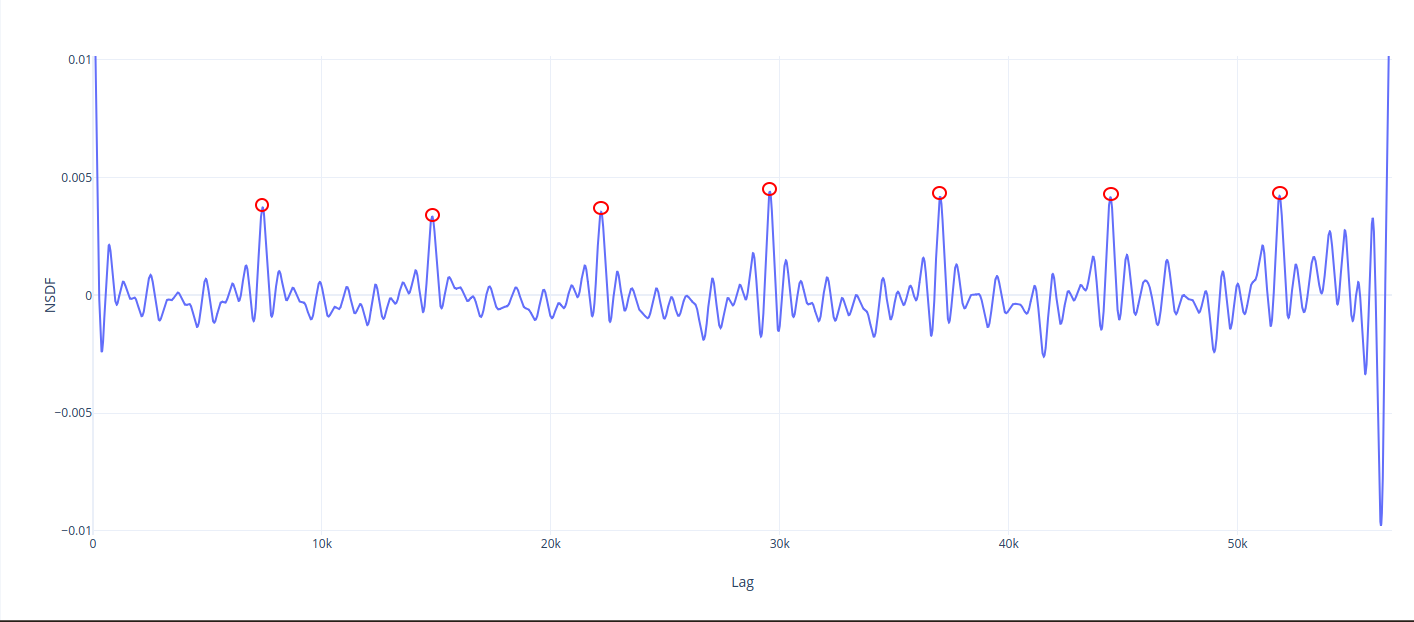
\includegraphics[width=.9\textwidth]{images/nsdf-dna-cut100.png}
}
\\
\subfloat[Raw signal\label{fig:mpm100_raw}]{
	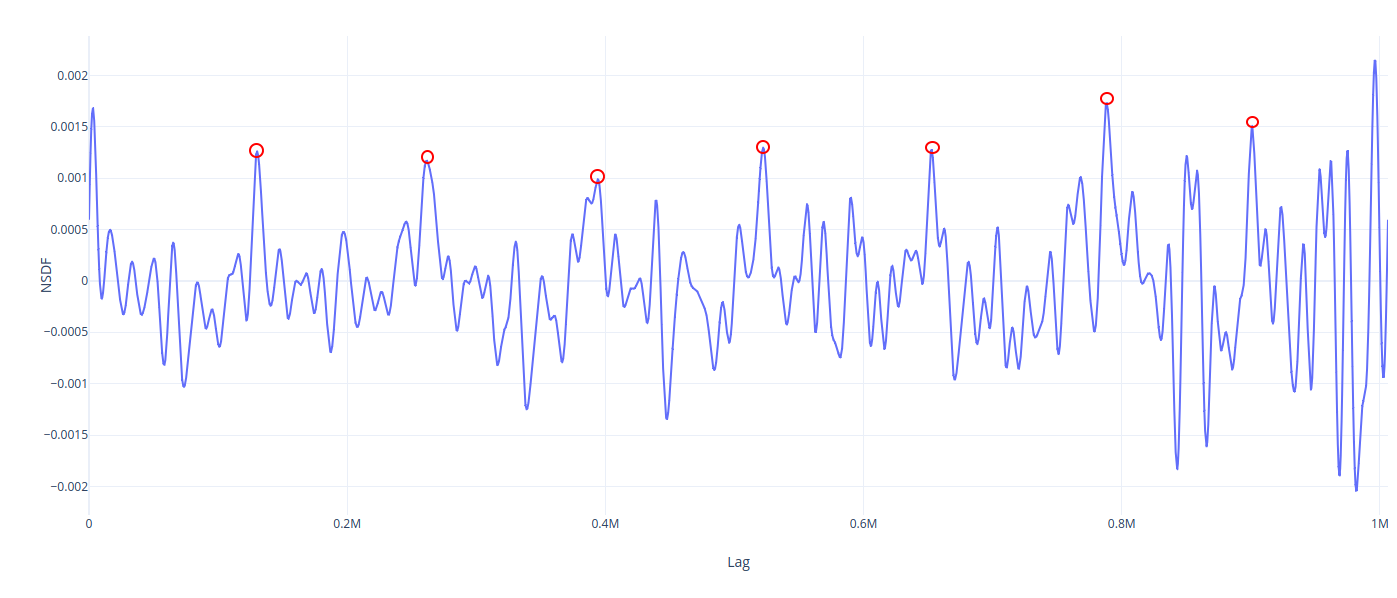
\includegraphics[width=.9\textwidth]{images/nsdf-raw-cut100.png}
}
\caption[Peak picking for a 7-concatemers NSDF signal processed with LPF using $cutFreq=100$]{Peak picking results for a 7-concatemers NSDF signal processed with LPF using $cutFreq=100$ of (\ref{fig:mpm100_dna}) the base-called DNA sequence and (\ref{fig:mpm100_raw}) its corresponding raw signal.}
\label{fig:mpm100}
\end{figure}

\paragraph{Pick peaking algorithm}
A list of candidates are first selected out of all local maxima by choosing the highest ones locating between every positively sloped zero crossing and negatively sloped zero crossing~\cite{Mcleod2005tartini}.
By setting the cutoff frequency, a respective minimum period (or monomer length) is determined as a consequence: $minLen=\frac{\displaystyle 1}{\displaystyle cutFreq}$. 
Any peaks on the left of this value will be ignored and the algorithm will iteratively scan to the right in the remaining peaks list for the correct first peak.
The correct first peak at $n_1$ must satisfy criteria as below:
\begin{itemize}
    \item[(1)] There are at least $\lfloor \frac{\displaystyle L}{\displaystyle n_1} \rfloor - 1$ more peaks with similar distances along the signal sequence.
    \item[(2)] The sum of these peaks' height must be more than a certain portion, \EG{} $0.8$, of the counterpart for all candidates.
\end{itemize}
The algorithm will stop at the very first coordinate that meets above 2 conditions and return the list of periodic peaks which can be used to break the concatemer into monomers. 

Figure~\ref{fig:mpm100} also reflects the peak-picking results applied for the longest concatemeric read. 
In both signal level, we detect exactly 7 peaks (highlighted in red dots) corresponding to the breakpoints that can be used for a $7$-concatemer chopping process.
Interestingly, when the peaks from DNA signal shows very stable repeat pattern, there is a slight variance from raw signal toward the far end. 
This phenomenon is shown clearer in Appendix Figure~\ref{supp_fig:mpm30_raw} when the sixth peak is shifted more to the right, considerably making the sixth monomer longer and the seventh monomer shorter than average.
We argue that there should be an unsmooth transition of the squiggle signal reading from the sequencing process~\cite{Rang2018squiggle}.
This is due to the nonuniform translocation time of the DNA molecule caused by the motor enzyme at the \emph{homopolymeric} regions~\cite{Manrao2012reading,Cherf2012automated,Sarkozy2017calling} and normally responsible for the high indels from nanopore sequencing~\cite{Jain2018nanopore3,Stancu2017nanopore5,Ip2015minion}.
However, the base-calling in this case has successfully manipulated the situation, resulting in more evenly-distributed peaks being detected.

Overall, via above example, we demonstrated that a 7-concatemer can be detected using the reference-free method based on NSDF signal investigation.
Similarly, any $k$-concatemer ($k \geq 1$) can be identified by the same manner and its monomers can be extracted by chopping at respective break-points. However, in order to obtain results of high confident, only reads corresponding to $k \geq 2$ should be selected as they would show more than 2 peaks for an affirmative picking task.
\section{Conclusion}
This chapter demonstrated a method of using MinION sequencing together with RCA for small-sized circular genomes, in particular two samples from \emph{Caulimovirids}.
Results from this preliminary finding showed that concatemer molecules generated from RCA can be sequenced directly by the thumbnail sequencer without using restriction enzymes to physically divide them into monomers. 

In fact, this step can be accomplished by using computational approaches, given or not a reference sequence.
In the reference-based method, corresponding monomers' break-points for RCA reads could be detected straightforward, resulting in abundance of single-copied sequences that could be subjected to a consensus calling.
For the \emph{de novo} detection algorithm, concatemeric reads were more confidently identified if they contains higher number of monomer duplication. For that reason, we can apply the reference-free method on data from CaMV barcoded sample to extract monomers and run the consensus calling with 35-folds coverage. RCA for BSMYV, on the other hand, returned solely monomers which were exclusively detectable given the reference DNA.
Further improvement from sequencing phase should be made in order to achieve longer stretches of clones so that the pipeline can operate completely without prior knowledge about the target genome.

The implemented module could operate rapidly read-by-read thus it is able to adapt for a streaming pipeline. For instance, a viral or plasmid sequencing would run until sufficient copies of monomers are produced for each sample.
Furthermore, the whole process can be established at raw signal level, before the base-calling step. 
For reference-based algorithm, the alignment step can be carried out between sequences of squiggle signal, as described in \emph{Read-Until} protocol~\cite{LooseMS2016}.
In case a reference is not provided, an DSP implementation based on NSDF is available for the task of determining concatemers.

In summary, this approach provide another promising method to study relative small but highly varied genomes of microorganisms. For instance, the longer concatemeric sequences will offer superior resolution to the nucleotides of individual virus thus enhancing the knowledge about inter- and intra-sample variations of this rapid evolving species. Continuing efforts are made to improve the monomer copy numbers from RCA reads so that we can utilize the methods in more comprehensive ways for real-life applications.